\documentclass[11pt]{article}
\usepackage{graphicx}
\usepackage[top=0.75in, bottom=1.75in, left=1in, right=1in,includefoot]
{geometry}
\usepackage{fancyhdr}
\usepackage[english]{babel}
\usepackage[math]{blindtext}
\usepackage{listings}
\usepackage{xcolor}
\usepackage{float}
\usepackage{amsmath}
\usepackage{amssymb}
\usepackage{mathpartir}
\usepackage{hyperref}
\usepackage{cleveref}
\usepackage{stmaryrd}
\usepackage[OT1]{fontenc}
\usepackage{utilities}
\usepackage{relsize}


\providecommand{\todo}[1]{\textcolor{red}{\textbf{TODO:} #1}}
\makeatletter
\@addtoreset{figure}{section}
\makeatother
\renewcommand{\thefigure}{\thesection.\arabic{figure}}
\newcommand{\List}{\mathsf{List}}
\newcommand{\LDispose}{\mathsf{LDispose}}
\newcommand{\LLen}{\mathsf{LLen}}
\newcommand{\CClist}{\mathsf{CClist}}
\newcommand{\CCllist}{\mathsf{CCllist}}
\newcommand{\addnode}{\mathsf{addnode}}
\newcommand{\reach}{\mathsf{reach}}
\newcommand{\Assert}{\mathsf{Assert}}
\newcommand{\True}{\mathsf{True}}
\newcommand{\False}{\mathsf{False}}
\newcommand{\Emp}{\mathsf{emp}}
\newcommand{\sepimp}{\mathrel{-\mkern-6mu\ast}}
\newcommand{\Eval}[1]{\mathcal{E}[\![#1]\!]_{e,s}}
\newcommand{\Val}{\mathsf{Val}}
\newcommand{\Heap}{\mathsf{Heap}}
\newcommand{\Pred}{\mathsf{pred}}
\newcommand{\pv}{\mathsf{pv}}
\newcommand{\Mod}{\mathsf{mod}}
\newcommand{\Bool}{\mathsf{Bool}}
\newcommand{\Var}{\mathsf{Var}}
\newcommand{\Exp}{\mathsf{Exp}}
\newcommand{\Null}{\mathsf{null}}
\newcommand{\blueassn}[1]{\textcolor{blue}{#1}}
\newcommand{\triple}[3]{\vdash\ \blueassn{\{#1\}}\ #2\ \blueassn{\{#3\}}}
\newcommand*{\defeq}{\mathrel{\vcenter{\baselineskip0.5ex \lineskiplimit0pt
                     \hbox{\scriptsize.}\hbox{\scriptsize.}}}%
                     =}
\newcommand*{\ddefeq}{\mathrel{\vcenter{\baselineskip0.5ex \lineskiplimit0pt
                     \hbox{\scriptsize.}\hbox{\scriptsize.}}}%
                      \mathrel{\vcenter{\baselineskip0.5ex \lineskiplimit0pt
                     \hbox{\scriptsize.}\hbox{\scriptsize.}}}
                     =\ }


\pagestyle{fancy}
\fancyhead[L]{\fancyhdrbox[c]{\Large \slshape \sffamily 
Separation Logic and Compositional Symbolic Execution:\\
Verification and Bug Detection at Scale}}
\fancyhead[C]{}
\fancyhead[R]{\large \sffamily \bfseries Philippa Gardner}
\fancyfoot[L]{\fancyhdrbox[b]{\sffamily \small Compiled By: \\ 
\normalsize \sffamily Dinghong Zhong, Samuel Dodson, Daniel Pinto}}
\fancyfoot[C]{\thepage}
\fancyfoot[R]{\fancyhdrbox[b]{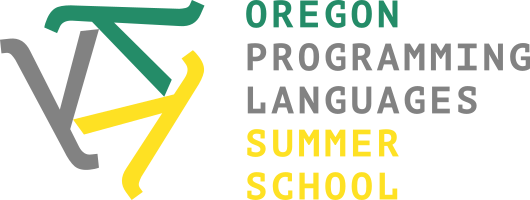
\includegraphics[width=1in]{oplssLogo.png}}}
\renewcommand{\footrulewidth}{0.5pt}

\fancypagestyle{plain}{
\fancyhf{}
\fancyfoot[L]{\fancyhdrbox[b]{\sffamily \small Compiled By: \\ 
Dinghong Zhong, Samuel Dodson, Daniel Andres Pinto Alvarado}}
}

\setlength{\parindent}{0pt}
\setlength{\parskip}{2ex}
\setlength{\headheight}{1.25in}
\setlength{\footskip}{32pt}
\begin{document}

\thispagestyle{plain}
\begin{center}
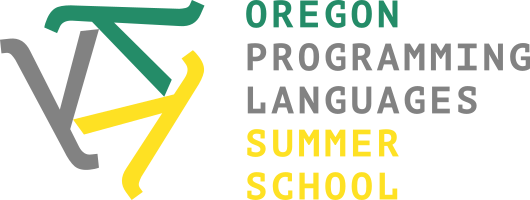
\includegraphics[width=3in]{oplssLogo.png}\\
\sffamily \LARGE \slshape 
Separation Logic and Compositional Symbolic Execution:\\
Semi-Automatic Verification and Automatic Bug Detection\\[2ex]
\upshape Philippa Gardner\\[2ex]
\large Lecture 4 - \slshape June 27, 2026
\end{center}

These are the notes for the fourth lecture of the OPLSS 2026 course on Separation Logic and Compositional Symbolic Execution, taught by Philippa Gardner. 
The official lecture slides are available at \url{https://gillianplatform.github.io/docs/oplss26/Lecture4.pdf}.

\section{Parametric Symbolic Execution}

Gillian\footnote{Project page and documentation: \url{https://gillianplatform.github.io/}.} is a general platform for building compositional program-analysis tools.
Its defining feature is that it is \emph{parametric on the partial symbolic state}: the engine is written once, against an algebraic interface, and the language-specific \emph{match}, \emph{consume}, and \emph{produce} algorithms are required to satisfy the laws of that interface.
Supplying an instance of the interface yields a tool for a particular language.
The platform has been instantiated as Gillian-JS and Gillian-C, and more recently as Gillian-Rust, which combines automated verification of safe Rust (via Creusot) with semi-automated verification of unsafe Rust.
Gillian has been used for both semi-automatic verification and automatic bug detection on real-world code, including the message-header deserialization module of the AWS Encryption SDK.

At the bottom of the picture is a single \emph{core symbolic-execution engine} for GIL, the Gillian Intermediate Language.
GIL is a small goto-style language; each target language is compiled down to GIL, and the engine executes GIL symbolically.
The engine is an interpreter: it walks the program and dispatches first-order \emph{path constraints} to an SMT solver exactly when they are needed (for example, to decide which branch of a conditional is feasible).
For efficiency it carries its own incremental SMT solver and falls back to Z3 only when required.

This engine deliberately leaves out memory semantics--loading and storing, checking that a pointer is valid in C, looking a field up along the prototype chain in JavaScript: none of these is fixed by the engine.
The engine knows how to drive control flow and talk to the solver, but it knows nothing about the shape of the heap it is manipulating. This is precisely what ``parametric'' means here, and it is what lets one engine serve many languages.
The hole is filled by supplying a \emph{memory model}, and the parametric soundness theorem guarantees that, provided the basic actions satisfy the interface, the resulting whole-program analysis is sound.

\textbf{Whole-program symbolic testing.} The first regime needs nothing more than the core engine plus a memory model.
The user annotates only \emph{first-order assertions about the symbolic inputs and outputs}.
On success it delivers \emph{bounded} correctness guarantees --- loops are unrolled to a fixed depth, so the verdict holds only up to that bound.
On failure it returns a \emph{concrete counter-model}/an actual input witnessing the violation.
This is automatic, whole-program bug-finding in the style of a bounded model checker such as CBMC.

\textbf{Compositional verification.}
The second regime adds a layer above the core engine: a \emph{compositional engine for separation-logic summaries}.
Rather than running a program whole, this engine can \emph{execute} separation-logic function specifications and loop invariants directly --- consuming a precondition and producing a postcondition at each call --- and it supports user-defined inductive predicates.
To make this work the memory model must be enriched with \emph{interpreted core predicates}: the primitive points-to assertion $x \mapsto y$ and friends, against which \emph{consume} matches.
Plugging in different interpreted core predicates is also what lets Gillian automate reasoning steps (lemmas) specific to a language.
The user now annotates separation-logic specifications, invariants, lemmas, and proof tactics; on success the guarantee is full \emph{functional correctness}, this time \emph{unbounded}; on failure the tool reports a \emph{failing symbolic trace}.
The consume/produce technique placing Gillian here is the same one underlying VeriFast and Viper.

\textbf{Automatic true bug-finding.} The third regime sits on a thin additional layer: a \emph{fix-from-error bi-abduction engine}, exposed through a small ``Fix API''.
Bi-abduction is the inference technique behind tools like Infer: on hitting a missing-resource error during symbolic execution, it abduces the precondition that would have been needed, simultaneously inferring the \emph{anti-frame} (the resource the code requires) and the \emph{frame} (the resource left over).
Run in the under-approximate direction, this turns each error into an inferred specification under which a \emph{genuine} fault is reachable, so the analysis needs \emph{no annotations at all}.
The trade-off is the reverse of verification: on success there is \emph{no guarantee} (a clean run does not certify correctness), but on failure there is a strong one --- a \emph{guarantee of a true bug}, with no false positives.
This is automatic, compositional, true bug-finding in the style of Meta's Infer Pulse, whose foundation is Incorrectness Separation Logic.

\end{document}
